%%%%%%%%%%%%%%%%%%%%% chapter.tex %%%%%%%%%%%%%%%%%%%%%%%%%%%%%%%%%
%
% sample chapter
%
% Use this file as a template for your own input.
%
%%%%%%%%%%%%%%%%%%%%%%%% Springer-Verlag %%%%%%%%%%%%%%%%%%%%%%%%%%

%\motto{Use the template \emph{chapter.tex} to style the various elements of your chapter content.}
\chapter{LTE-Advanced: An Overview}
\label{overview-lte} % Always give a unique label
% use \chaptermark{}
% to alter or adjust the chapter heading in the running head

\abstract*{This chapter provides a high-level overview of LTE-Advanced (LTE-A) networks and associated technologies to form a basis for discussion of the coexistence issues that exist for unlicensed LTE and \mbox{Wi-Fi}. Understanding the underlying architecture and protocols employed in LTE-A networks will provide a comparative framework to grasp how, and at what levels, LTE and \mbox{Wi-Fi} networks may interact and interfere with each other, and form a greater understanding of the challenges to be address in designing coexistence mechanisms. Specifically, this chapter will overview the LTE-A network, as well as its capabilities and protocols, with specific emphasis on the physical layer and medium access sub-layers to illuminate specific sources of coexistence issues. Proposed changes which may be included in future LTE releases are discussed in the context of LTE/\mbox{Wi-Fi} coexistence.}

This chapter provides a high-level overview of LTE-Advanced (LTE-A) networks and associated technologies to form a basis for discussion of the coexistence issues that exist for unlicensed LTE and \mbox{Wi-Fi}. Understanding the underlying architecture and protocols employed in LTE-A networks will provide a comparative framework to grasp how, and at what levels, LTE and \mbox{Wi-Fi} networks may interact and interfere with each other, and form a greater understanding of the challenges to be address in designing coexistence mechanisms. Specifically, this chapter will overview the LTE-A network, as well as its capabilities and protocols, with specific emphasis on the physical layer and medium access sub-layers to illuminate specific sources of coexistence issues. Proposed changes which may be included in future LTE releases are discussed in the context of LTE/\mbox{Wi-Fi} coexistence.


\section{System Overview}
\label{sys-overview}
The enhancements to the Long Term Evolution/System Architecture Evolution (LTE/SAE) to meet the requirements set out for fourth generation (4G) cellular networks are collectively known as LTE-Advanced (\mbox{LTE-A}).  The \mbox{LTE-A} requirements were formalized by the 3rd Generation Partnership Project (3GPP) in LTE releases 10 through 13 \cite{tr36913}.  LTE itself was a logical evolution from the technologies used in previous generations in order to meet the increasing demands for higher data rates and improved quality of service. LTE met these demands at the access level through increased spectral efficiency and improved mobility support and cell edge data rates.  The increased spectral efficiency was achieved by using orthogonal frequency division multiple access (OFDMA) and single-carrier frequency division multiple access (SC-FDMA) in the downlink (DL) and uplink (UL), respectively.  Improvements in mobility support and cell edge data rates were achieved through enhanced adaptive modulation and bandwidth selection and DL spatial multiplexing and multiple input/multiple output support.  Beyond the access layer, LTE transitioned to an all-IP packet switched core network with the introduction of the evolved packet core, and a flattened network architecture of enhanced base stations called evolved NodeB's (eNB) interconnected via high-speed data links.  Combined, these fundamental changes to the cellular network architecture have allowed LTE networks to significantly increase user data rates and reduce control and user plane latency and connection set-up and handover times.  \mbox{LTE-A} represents the further, and ongoing, evolution of cellular networks to continue to meet the ever-increasing demands for higher data rates, user mobility support, and efficient support of a growing number of wireless devices.

\subsection{Network Architecture}
\label{net-arch}
The requirements to provide high data rates while supporting high-speed mobility requires the ability to set up and tear down user connections and manage inter-cell handoffs with as little latency as possible.  In previous generations of cellular networks, a hierarchical structure consisting of base stations or NodeBs connected to a central controller had been used.  This star or cluster architecture requires additional hops in both data transmissions and hand off negotiation which can introduce significant delay.  Controllers were responsible for managing all data and control traffic as well as handoffs betweens several pairs of base stations.  For many increasingly ubiquitous end-user applications, such as online gaming and voice/video over the internet, the additional latency in connection set up and handover can impair the user-perceived quality of experience.
\begin{figure}[!ht]
	\centering
	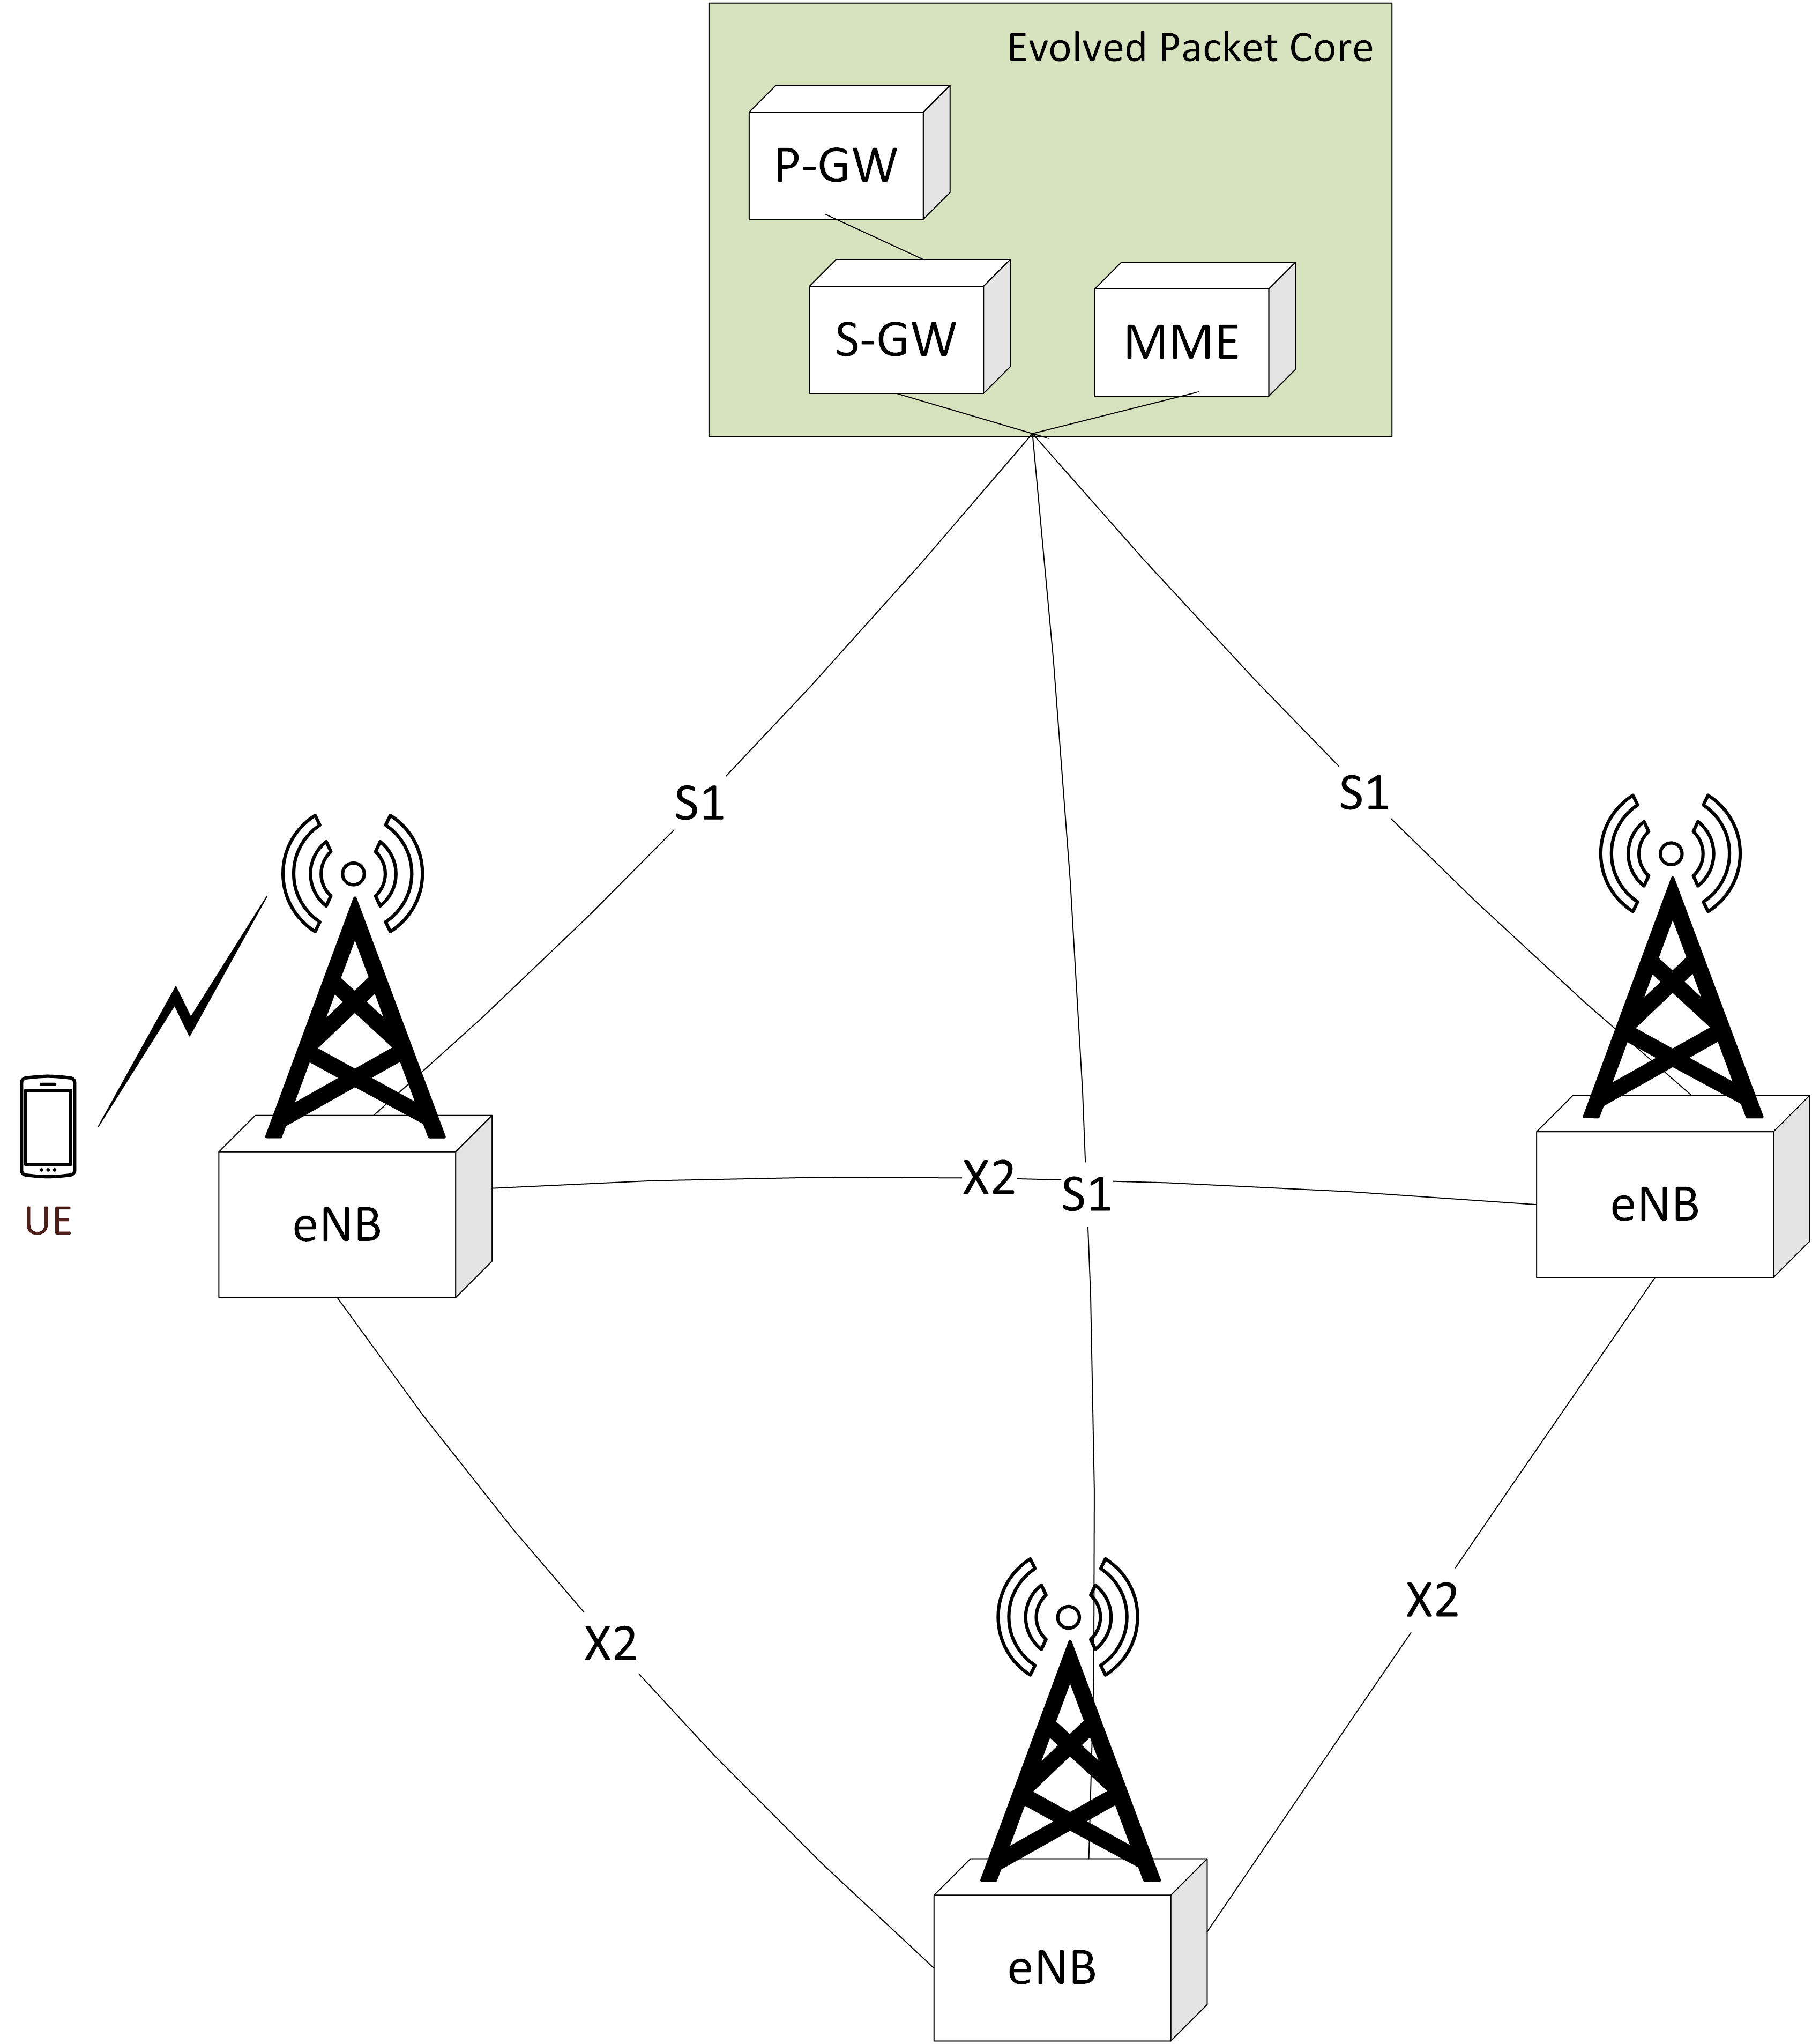
\includegraphics[width=0.58\textwidth]{figs/lteAnet}
	\caption{Basic structure of LTE cellular networks.}
	\label{figs:LTE-A-Network}
\end{figure}

The flat architecture adopted by LTE networks is depicted in Fig. \ref{figs:LTE-A-Network}.  The migration of local functions to eNBs and global functions to the EPC were driven by the requirements of reduced latency and higher data rates. The functions of radio network and medium access control, handoff requests, negotiations, and management, as well as some other truly local functions, are migrated to the eNBs \cite{tr36300}. The eNBs interconnected via the low-latency X2 interface connections between eNBs in a mesh configuration to allow for fast user handover, including forwarding of queued data for seamless user experience.  Additionally, with direct connections between neighboring cells, this architecture facilitates more effective multi-point transmission, coordination, and inter-cell interference and load management, independent of conditions in other areas of the network. The global functions and connections to external networks are handled at the evolved packet core (EPC). The functional split between the various components of the network, as well as the implementation of the necessary layers of the network protocol stack, is shown in further detail in Fig. \ref{figs:funcSplit}.
\begin{figure}[!ht]
	\centering
	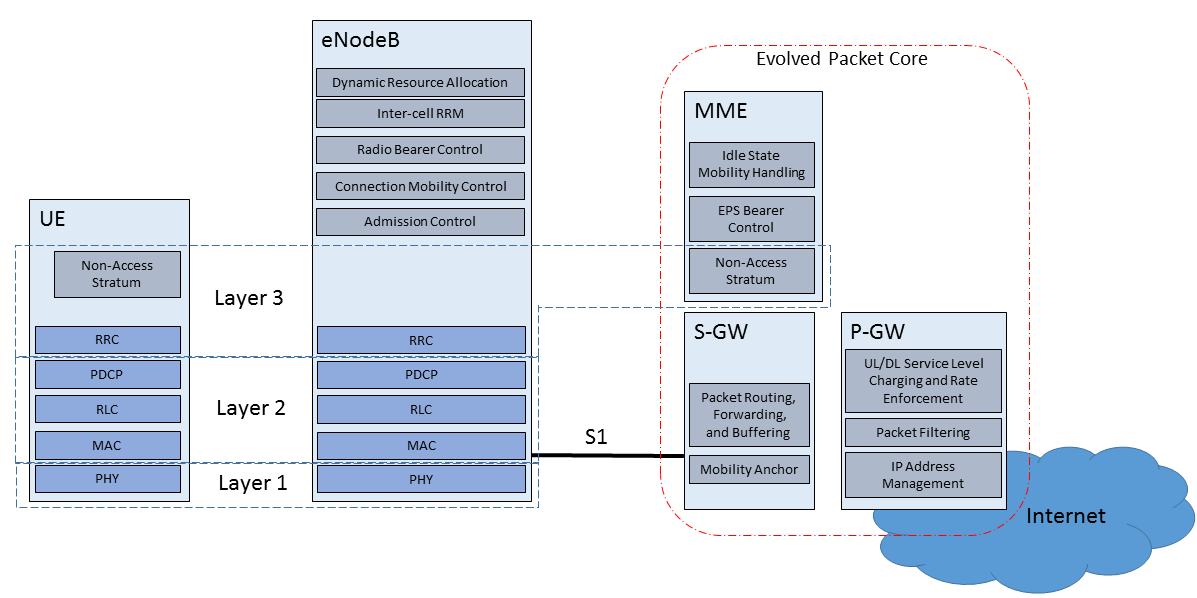
\includegraphics[width=\textwidth]{figs/LTE-decomp}
	\caption{Functional split between various entities in LTE under the system architecture evolution.}
	\label{figs:funcSplit}
\end{figure}
In addition to those functions listed in the figure, the mobile management entity (MME) handles authentication, authorization and accounting functions.  The packet data network gateway (P-GW) and serving gateway (S-GW) handle user data packet forwarding, filtering, and usage tracking, as well as acting as a mobility anchor for inter-eNB and inter-RAT handovers.  Further, the distributed radio network and resource management and medium access control allows eNBs to quickly adapt to changing radio medium conditions and provide timely user scheduling based on local information.

\subsection{Capabilities and Features}

While the gains made by LTE were significant, they fell short of the requirements set out for 4G networks by the International Telecommunications Union, specifically in the case of peak data rates, spectral efficiency, and cell edge performance \cite{itu-advanced}.  The continuing evolution which became \mbox{LTE-A} was finally able to achieve the necessary targets to meet the ITU requirements for 4G.  Some important ITU requirements, and achieved performance levels for LTE and \mbox{LTE-A}, are highlighted in Table \ref{perf-table}.

\begin{table}
	\caption{ITU-A Requirements for 4G vs. LTE/\mbox{LTE-A} Achievements \cite{lte-3gpp}\cite{lteA-3gpp}\cite{itu-advanced}\cite{abdullah}}
	\label{perf-table}      
	\begin{tabular}{p{0.5\textwidth}p{0.15\textwidth}p{0.15\textwidth}p{0.15\textwidth}}
		\hline\noalign{\smallskip}
		Description/Requirements & ITU-A & LTE & \mbox{LTE-A}   \\
		\noalign{\smallskip}\svhline\noalign{\smallskip}
		DL peak spectral efficiency (bps/Hz) &  15   & 15  & 30 \\
		UL peak spectral efficiency (bps/Hz)& 6.75  & 3.75  & 15 \\
		Min. cell edge spectral \\ \hspace{0.8em} efficiency (bps/Hz) & 0.04 & 0.024 & 0.04 \\
		DL Peak data rates (Mbps) & 1000$^1$  & 300 & 1000 \\
		UL Peak data rates (Mbps) & 1000$^1$  & 75 & 500 \\
		Scalable bandwidth up to (MHz) & 40 & 20  & 100$^2$ \\
		
		\noalign{\smallskip}\hline\noalign{\smallskip}
	\end{tabular}
	$^1$ For low mobility with requirement of min. 100 Mbps for speeds of up to 350 km/h. 	 \\
	$^2$ With carrier aggregation of up to five carrier components.
\end{table}

Among other innovations, \mbox{LTE-A} extended bandwidth scalability in LTE by supporting carrier aggregation, both within and across frequency bands.   Discontiguous aggregation is supported to ensure a higher bandwidth is available for providers who cannot support it in contiguous spectrum allotments, allowing the development of license-assisted access (\mbox{LAA-LTE}) into the unlicensed and TV whitespace bands.  Backwards compatibility is maintained by using bandwidths for each carrier component which match those used in LTE.  \mbox{LTE-A} also expands MIMO/spatial multiplexing support up to 8x8 for DL and 4x4 for UL, adds coordinated multi-point operation to increase spectral efficiency and cell edge data rates, and improves heterogeneous network planning with the enhancement of support for small cells and relay nodes to increase area coverage with reduced power requirements.

\section{Channel Access Mechanisms}
\label{channel-access}
Like other cellular access technologies, \mbox{LTE-A} has been designed for use on dedicated licensed spectrum allocations where there is, generally, no need to contend for channel access.  While interference, fading, and path loss can corrupt LTE transmissions, and recovery and retransmission functions are necessary, in general a centrally controlled and tightly scheduled channel access mechanism is able to guarantee service levels required by all UL and DL traffic \cite{tr36300}. UL/DL separation is achieved through either time-division duplexing (TDD) or frequency-division duplexing (FDD).  Orthogonal frequency-division multiple access (OFDMA) is used in the DL, allowing the eNB to efficiently schedule transmissions for many users in the same transmission time interval.  Single-carrier frequency-division multiple access (SC-FDMA) is used in the uplink in order to reduce the power consumption requirements of battery-dependent user equipment (UE) to communicate with the eNB.  Further, coordinated multipoint (CoMP) is supported by allowing UEs to be configured to process channel state information (CSI) from multiple eNBs, and both single-user (SU) and multi-user (MU) MIMO are supported in multiple configurations to achieve transmit diversity or multi-layer transmissions with beamforming possible in both horizontal and vertical dimensions.

The basic structure of the protocol stack used in LTE networks to facilitate channel access is shown in Fig. \ref{figs:stack} \cite{tr36201}.
\begin{figure}[!ht]	
	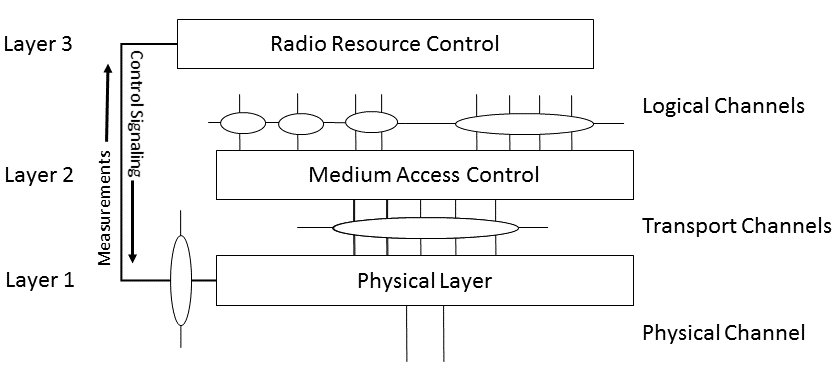
\includegraphics[width=\textwidth]{figs/LTEradio-interface}
	\caption{E-UTRA radio interface protocol architecture.}
	\label{figs:stack}
\end{figure}
UL and DL transmissions are divided amongst several physical channels, according to the type of transmission, i.e. user traffic or control information, and the type of transmission, i.e. broadcast or unicast and scheduled or random access (random access is primarily used by a UE which has not yet associated to an eNB). The information-bearing physical channels are mapped by the PHY layer into transport channels supplied to the MAC sublayer, which in turn remaps these into several logical channels provided to the higher layers. 

\subsection{\mbox{LTE-A} Physical Layer}
\label{lte-phy}
The LTE PHY layer is designed to be both highly adaptable as well spectrally and power efficient.  In the DL, OFDMA is used to schedule many signals in the same transmission time interval and achieve a high spectral efficiency; however, the very high peak to average power ratio makes this multiple access strategy unattractive in the UL for battery-dependent devices \cite{tr36201}\cite{tr36211}.  SC-FDMA is used in the UL to maintain a satisfactory spectral efficiency while significantly improving power efficiency and battery life. Example carrier allocations for both DL and UL are shown in Fig. \ref{lte:of-sc-fdma}.
\begin{figure}[!ht] 	
	\subfloat[OFDMA used in downlink.]{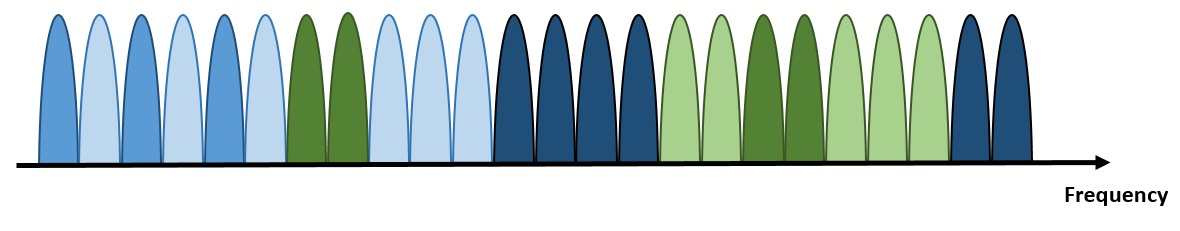
\includegraphics[width=\textwidth]{figs/ofdma}%
		\label{ofdma}}
	\\
	\subfloat[SC-FDMA used in uplink.]{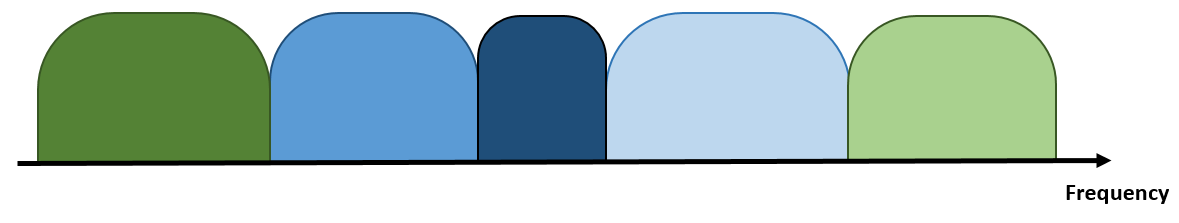
\includegraphics[width=\textwidth]{figs/sc-fdma}%
		\label{sc-fdma}}
	\caption{Multiple access strategies used in LTE for uplink and downlink.}
	\label{lte:of-sc-fdma}
\end{figure}
Each color and shade represents the carriers allocated to a specific user.  The assignment of sub-carriers to a given UE are driven by the specific loss and interference experienced by that user, called channel state information (CSI), in order to maximize the overall achieved rate of all users.  As shown in Fig. \ref{ofdma}, in the DL \mbox{LTE-A} supports both localized (contiguous) and distributed allocations, to best use CSI to maximize network efficiency. Sub-carrier assignments can further span disjoint frequency bands, including into unlicensed bands.  Fig. \ref{sc-fdma} depicts an example UL allocation where a given sub-carrier, with variable bandwidth, is assigned to a single UE, again based on CSI.  It should be emphasized that Fig. \ref{lte:of-sc-fdma} shows a single instant of time, over a subset of the available carriers in the band.

All transmissions are organized into frames comprised of twenty slots, every two of which comprise a subframe \cite{tr36211}. An example of one configuration for the LTE frame structure is shown in Fig. \ref{lte:frame}.
\begin{figure}[!t]
	\centering
	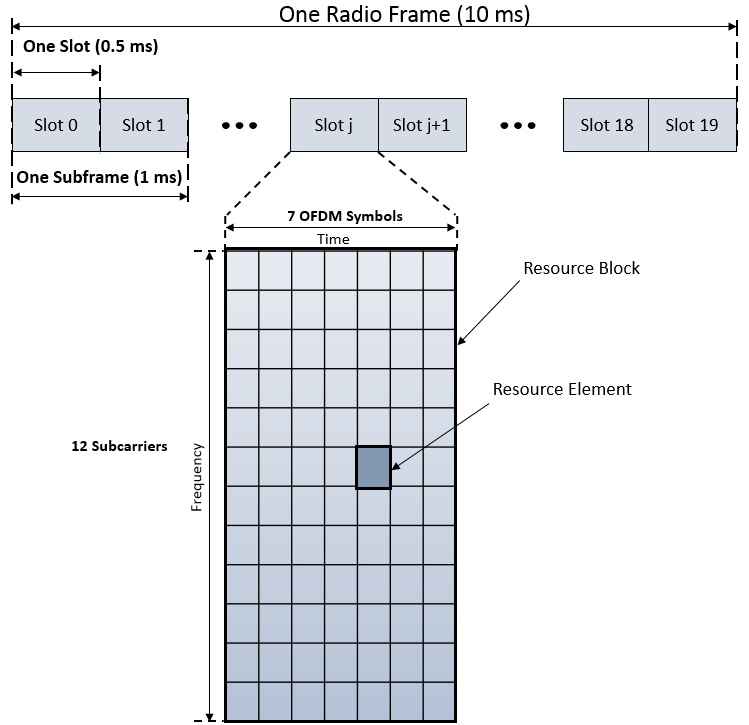
\includegraphics[width=0.8\textwidth]{figs/LTE-frame}
	\caption{LTE frame and resource block structure.}
	\label{lte:frame}
\end{figure}
A single sub-carrier, with either 7.5 or 15 kHz bandwidth, paired with a transmission duration required to transmit a single OFDM symbol is called a resource element.  The minimum unit which can be allocated to a physical channel or user is the physical resource block (PRB).  For simplicity, in the breakout, a single PRB is depicted, though a single PRB spans only a small subset of the available sub-carriers. Depending on the configuration used, a PRB is formed of either 3, 7, or 7 OFDM symbols and 12 or 24 sub-carriers allocated for one 0.5 ms slot.  Between 6 and 10 PRBs will then be allocated to a UE in order to achieve bandwidths between 1.4 and 20 MHz (though the occupied bandwidth will be smaller, 1.08 to 18 MHz).  Higher bandwidths are achieved through carrier aggregation in the same slot, either contiguous or not. 

Two distinct frame structures are defined to support both time division duplexing (TDD) and frequency division duplexing (FDD), as well as a third frame structure specifically for license assisted access (\mbox{LAA-LTE}).  All three frame types have the same basic structure shown in Fig. \ref{lte:frame}, with the differences being in how transmission are scheduled.  Both half- and full-duplex are supported in FDD and all 10 subframes are available for both UL and DL.  In half-duplex configurations, transmission are separated in both time and frequency, while for full-duplex transmissions separation is in frequency only.  For TDD, the frame is organized into two 5 ms half-frames, with several UL/DL configurations and switching patterns supported.  As of Release 13, the special frame structure defined for \mbox{LAA-LTE} reserves all 10 subframes for DL, with transmission able to occupy one or more consecutive subframes, but required to start somewhere within the first subframe. \mbox{LAA-LTE} is expected to be expanded to support both UL and DL in future releases.

Beyond the features discussed in detail, the \mbox{LTE-A} PHY layer provides forward error correction and automatic repeat request functions, modulation/demodulation of physical signals, mapping and rate matching of physical channels to transport channels, frequency and time synchronization, and MIMO antenna processing, including transmit diversity and beamforming.  A variety of modulation schemes are supported depending on channel conditions, distance from receiver, and power requirements (up to 256 QAM in the DL).  

\subsection{\mbox{LTE-A} Medium Access Control}
\label{lte-mac}
Medium access in LTE is tightly controlled and scheduled in both UL and DL, with the eNB controlling the time and frequency resource block assignment for all but random access channels (used for UE connection requests and some other procedures) \cite{tr36321}.  Distinct MAC sub-layers for the eNB and the UE are defined, with each optimized to their specific functions and resources.  Additionally, several MAC configurations are defined for UE depending on the specific functions implemented, such as dual connectivity to support coordinated multipoint (CoMP) transmission and sidelink channels for UE device-to-device communication. The basic structure of the MAC sub-layer, without CoMP or sidelink configured, is shown in Fig. \ref{figs:lte-mac}.
\begin{figure}[!ht]
	\centering
	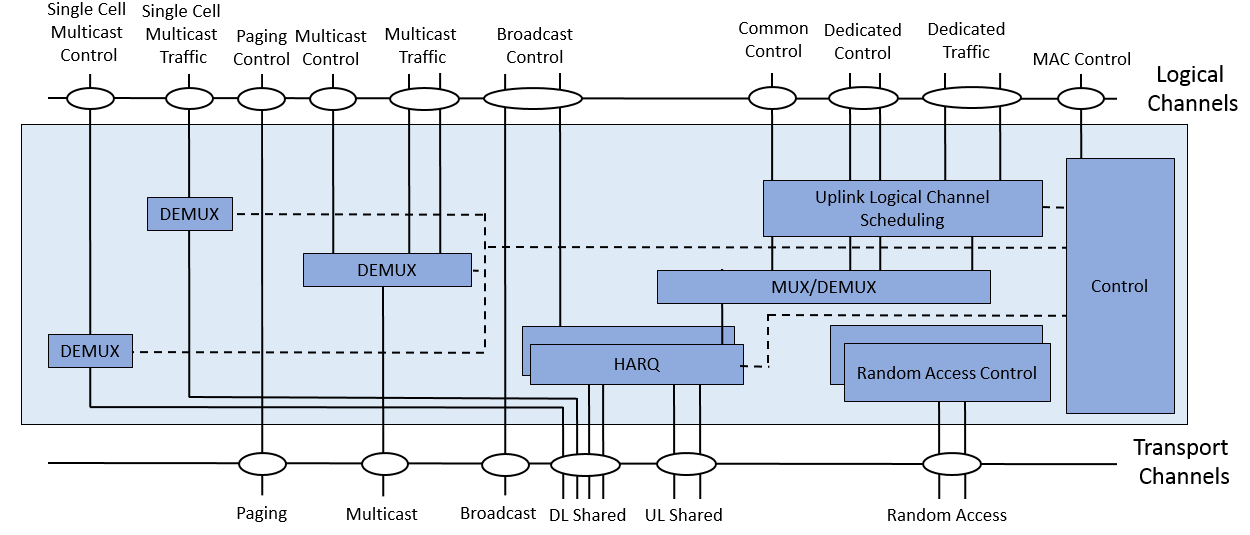
\includegraphics[width=\textwidth]{figs/LTE-MAC}	
	\caption{LTE MAC sublayer structure and channel mapping.}
	\label{figs:lte-mac}
\end{figure}
The extension to other MAC configurations requires the duplication of this basic structure, and separate control and traffic channels required. In dual connectivity, for example, two such MAC structures are implemented for the master and secondary cell group; however, only the broadcast, shared UL and DL, and random access channels are needed for the secondary cell group.  In sidelink configuration, only broadcast, discovery, and duplex UL/DL shared channels are required.

The MAC sub-layer facilitates reliable data transfer through radio resource allocation, UL traffic prioritization in the UE, and the mapping and multiplexing between transport channels and one or more logical channels. Further, the MAC sub-layer handles hybrid automatic repeat requests (HARQ) signaling, a combination of forward error correcting coding and error detection, as well as channel prioritization with dynamic scheduling, random access control, and scheduling information reporting and requests.

The specific implementation of these, and other layer 2 functions such as radio link control, are quite complex and beyond the scope of this brief; however, the underlying design paradigm is that of global knowledge facilitating tight control over medium access. The MAC sub-layer in the eNB is aware of the channel conditions for each UE to be scheduled in both the UL and DL, and the UE adheres to the schedule of time and frequency provided by the eNB.  PRBs are assigned to UL and DL transmissions to achieve the greatest advantage from local channel conditions. Little consideration of inter-user or inter-carrier interference is necessary, due to the dedicated frequency bands and orthogonal carriers discussed in Sec. \ref{lte-phy}.  As a result, \mbox{LTE-A} is able to achieve high spectral efficiency and reliability.


\section {Changes Expected for Future Releases}
\label{fut-chnge}
\mbox{LTE-A} brings cellular networks into the realm of 4G, as defined by \cite{itu-advanced}.  As far as \mbox{LTE-A} has taken us, it will not be enough for fifth generation (5G) networks which are expected to support existing and new use cases ranging from smart cities and Internet of Things devices (massive machine type communication) to self-driving vehicles and industrial automation (ultra-reliable and low latency communications) with  high speed mobile broadband on the order of giga\emph{bytes} per second \cite{itu-2020}.  Some of the specific requirements are outlined in Table \ref{5g-table}.
\begin{table}
	\caption{ITU-A Requirements for 4G vs. ITU-2020 Requirements for 5G  \cite{itu-2020}}
	\label{5g-table}      
	\begin{tabular}{p{0.6\textwidth}p{0.18\textwidth}p{0.18\textwidth}}
		\hline\noalign{\smallskip}
		Description/Requirements & ITU-A & ITU-2020  \\
		\noalign{\smallskip}\svhline\noalign{\smallskip}
		Peak data rates (Gbps) & 1  & 20\\
		Average user data rates (Mbps) & 1  & 100  \\				
		Mobility support(km/h) & 350  & 500 \\
		Connection density (devices/km$^2$ )& 10$^5$ & 10$^6$ \\
		Traffic capacity (Mbits/s/m$^2$) & 0.1 & 10 \\
		\noalign{\smallskip}\hline\noalign{\smallskip}
	\end{tabular}
		
\end{table}
Beyond these specific targets set by the ITU, 5G networks must also achieve 10$\times$ reduced latency, 3$\times$ improved spectral efficiency and  100$\times$ network energy efficiency, compared to 4G networks. 

In order to move towards 5G networks, 3GPP has numerous study items underway and planned for future releases, to meet the ITU requirements in \cite{itu-2020}.  These include significant enhancements to inter- and intra-band carrier aggregation and licenses-assisted access to ISM bands, TV white space, and other under-utilized spectrum resources, as well as multi-carrier enhancements and improved CoMP and device-to-device communications \cite{lteA-gantt}.  Wireless network virtualization and hardware resource sharing, cloud-based radio access networks, and new system architectures are under consideration to support the requirements around energy efficiency and low-latency communications, among others.  Additionally, the possibility of moving to entirely new radio and medium access protocols is also under consideration, which would not be hindered by the need to be backwards compatible, and move forward with only the necessity of meeting the ITU 5G requirements. 

%%%%%%%%%%%%%%%%%%%%%%%% referenc.tex %%%%%%%%%%%%%%%%%%%%%%%%%%%%%%
% sample references
% %
% Use this file as a template for your own input.
%
%%%%%%%%%%%%%%%%%%%%%%%% Springer-Verlag %%%%%%%%%%%%%%%%%%%%%%%%%%

\begin{thebibliography}{99.}%
	\bibitem{tr36913}{3GPP}, ``{Requirements for further advancements for Evolved Universal Terrestrial Radio Access (E-UTRA) (LTE-Advanced)},'' \emph{{3GPP TR 36.913 version 13.0.0 Release 10}}, 2011.
	\bibitem{tr25.913}{3GPP}, ``{Requirements for evolved UTRA (E-UTRA) and evolved UTRAN (E-UTRAN)},'' \emph{{3GPP TR 25.913 version 8.0.0 Release 8}}, 2009.
	\bibitem{tr36321}{3GPP}, ``{Evolved universal terrestrial radio access (E-UTRA); Medium access control (MAC) protocol specification},'' \emph{{3GPP TS 36.321 version 13.1.0 Release 13}}, 2016.
	\bibitem{tr36300}{3GPP}, ``{Evolved universal terrestrial radio access (E-UTRA) and evolved universal terrestrial radio access network (E-UTRAN); Overall description},'' \emph{{3GPP TS 36.300 version 13.3.0 Release 13}}, 2016.
	\bibitem{tr36201}{3GPP}, ``LTE; Evolved universal terrestrial radio access (E-UTRA); Physical layer; General description,'' \emph{{3GPP TS 36.201 version 13.1.0 Release 13}}, 2016.
	\bibitem{tr36211}{3GPP}, ``LTE; Evolved universal terrestrial radio sccess (E-UTRA); Physical channels and modulation,'' \emph{{3GPP TS 36.211 version 13.1.0 Release 13}}, 2016.
	\bibitem{lte-3gpp}{3GPP}, ``{LTE},'' Whitepaper, ND. Accessed: June 21, 2016 [Online]. Available: \url{{www.3gpp.org/technologies/keywords-acronyms/98-lte}}
	\bibitem{lteA-3gpp}{3GPP}, ``{LTE-Advanced},'' Whitepaper, June 2013. Accessed: June 21, 2016 [Online]. Available: \url{{www.3gpp.org/technologies/keywords-acronyms/97-lte-advanced}}
	\bibitem{lteA-gantt}{3GPP}, ``{3GPP work programme (and associated reference links therein)},'' July 2016. Accessed: July 12, 2016 [Online]. Available: \url{{www.3gpp.org/dynareport/GanttChart-Level-2.htm}}		
	\bibitem{itu-advanced}{ITU}, ``IMT Vision –	Framework and overall objectives of the future development of IMT for 2020 and beyond,'' \emph{Rep. ITU-R M.2083-0}, 2015. 
	\bibitem{itu-2020}{ITU}, ``Requirements related to technical performance for IMT-Advanced radio interface(s),'' \emph{Rep. ITU-R M.2134}, 2008. 
	\bibitem{abdullah} {M.F.L. Abdullah and A.Z. Yonis}, ``{Performance of LTE release 8 and release 10 in wireless communications},'' in \emph{{Cyber Security, Cyber Warfare and Digital Forensic (CyberSec), 2012 International Conference on}}, June 2012, pp. 236--241.
		
\end{thebibliography}
